% Options for packages loaded elsewhere
\PassOptionsToPackage{unicode}{hyperref}
\PassOptionsToPackage{hyphens}{url}
%
\documentclass[
]{article}
\usepackage{amsmath,amssymb}
\usepackage{lmodern}
\usepackage{iftex}
\ifPDFTeX
  \usepackage[T1]{fontenc}
  \usepackage[utf8]{inputenc}
  \usepackage{textcomp} % provide euro and other symbols
\else % if luatex or xetex
  \usepackage{unicode-math}
  \defaultfontfeatures{Scale=MatchLowercase}
  \defaultfontfeatures[\rmfamily]{Ligatures=TeX,Scale=1}
\fi
% Use upquote if available, for straight quotes in verbatim environments
\IfFileExists{upquote.sty}{\usepackage{upquote}}{}
\IfFileExists{microtype.sty}{% use microtype if available
  \usepackage[]{microtype}
  \UseMicrotypeSet[protrusion]{basicmath} % disable protrusion for tt fonts
}{}
\makeatletter
\@ifundefined{KOMAClassName}{% if non-KOMA class
  \IfFileExists{parskip.sty}{%
    \usepackage{parskip}
  }{% else
    \setlength{\parindent}{0pt}
    \setlength{\parskip}{6pt plus 2pt minus 1pt}}
}{% if KOMA class
  \KOMAoptions{parskip=half}}
\makeatother
\usepackage{xcolor}
\IfFileExists{xurl.sty}{\usepackage{xurl}}{} % add URL line breaks if available
\IfFileExists{bookmark.sty}{\usepackage{bookmark}}{\usepackage{hyperref}}
\hypersetup{
  pdftitle={Final Report: Selling to both Sides (Moore 2012)},
  pdfauthor={Carlo Greß},
  hidelinks,
  pdfcreator={LaTeX via pandoc}}
\urlstyle{same} % disable monospaced font for URLs
\usepackage[margin=1in]{geometry}
\usepackage{color}
\usepackage{fancyvrb}
\newcommand{\VerbBar}{|}
\newcommand{\VERB}{\Verb[commandchars=\\\{\}]}
\DefineVerbatimEnvironment{Highlighting}{Verbatim}{commandchars=\\\{\}}
% Add ',fontsize=\small' for more characters per line
\usepackage{framed}
\definecolor{shadecolor}{RGB}{248,248,248}
\newenvironment{Shaded}{\begin{snugshade}}{\end{snugshade}}
\newcommand{\AlertTok}[1]{\textcolor[rgb]{0.94,0.16,0.16}{#1}}
\newcommand{\AnnotationTok}[1]{\textcolor[rgb]{0.56,0.35,0.01}{\textbf{\textit{#1}}}}
\newcommand{\AttributeTok}[1]{\textcolor[rgb]{0.77,0.63,0.00}{#1}}
\newcommand{\BaseNTok}[1]{\textcolor[rgb]{0.00,0.00,0.81}{#1}}
\newcommand{\BuiltInTok}[1]{#1}
\newcommand{\CharTok}[1]{\textcolor[rgb]{0.31,0.60,0.02}{#1}}
\newcommand{\CommentTok}[1]{\textcolor[rgb]{0.56,0.35,0.01}{\textit{#1}}}
\newcommand{\CommentVarTok}[1]{\textcolor[rgb]{0.56,0.35,0.01}{\textbf{\textit{#1}}}}
\newcommand{\ConstantTok}[1]{\textcolor[rgb]{0.00,0.00,0.00}{#1}}
\newcommand{\ControlFlowTok}[1]{\textcolor[rgb]{0.13,0.29,0.53}{\textbf{#1}}}
\newcommand{\DataTypeTok}[1]{\textcolor[rgb]{0.13,0.29,0.53}{#1}}
\newcommand{\DecValTok}[1]{\textcolor[rgb]{0.00,0.00,0.81}{#1}}
\newcommand{\DocumentationTok}[1]{\textcolor[rgb]{0.56,0.35,0.01}{\textbf{\textit{#1}}}}
\newcommand{\ErrorTok}[1]{\textcolor[rgb]{0.64,0.00,0.00}{\textbf{#1}}}
\newcommand{\ExtensionTok}[1]{#1}
\newcommand{\FloatTok}[1]{\textcolor[rgb]{0.00,0.00,0.81}{#1}}
\newcommand{\FunctionTok}[1]{\textcolor[rgb]{0.00,0.00,0.00}{#1}}
\newcommand{\ImportTok}[1]{#1}
\newcommand{\InformationTok}[1]{\textcolor[rgb]{0.56,0.35,0.01}{\textbf{\textit{#1}}}}
\newcommand{\KeywordTok}[1]{\textcolor[rgb]{0.13,0.29,0.53}{\textbf{#1}}}
\newcommand{\NormalTok}[1]{#1}
\newcommand{\OperatorTok}[1]{\textcolor[rgb]{0.81,0.36,0.00}{\textbf{#1}}}
\newcommand{\OtherTok}[1]{\textcolor[rgb]{0.56,0.35,0.01}{#1}}
\newcommand{\PreprocessorTok}[1]{\textcolor[rgb]{0.56,0.35,0.01}{\textit{#1}}}
\newcommand{\RegionMarkerTok}[1]{#1}
\newcommand{\SpecialCharTok}[1]{\textcolor[rgb]{0.00,0.00,0.00}{#1}}
\newcommand{\SpecialStringTok}[1]{\textcolor[rgb]{0.31,0.60,0.02}{#1}}
\newcommand{\StringTok}[1]{\textcolor[rgb]{0.31,0.60,0.02}{#1}}
\newcommand{\VariableTok}[1]{\textcolor[rgb]{0.00,0.00,0.00}{#1}}
\newcommand{\VerbatimStringTok}[1]{\textcolor[rgb]{0.31,0.60,0.02}{#1}}
\newcommand{\WarningTok}[1]{\textcolor[rgb]{0.56,0.35,0.01}{\textbf{\textit{#1}}}}
\usepackage{graphicx}
\makeatletter
\def\maxwidth{\ifdim\Gin@nat@width>\linewidth\linewidth\else\Gin@nat@width\fi}
\def\maxheight{\ifdim\Gin@nat@height>\textheight\textheight\else\Gin@nat@height\fi}
\makeatother
% Scale images if necessary, so that they will not overflow the page
% margins by default, and it is still possible to overwrite the defaults
% using explicit options in \includegraphics[width, height, ...]{}
\setkeys{Gin}{width=\maxwidth,height=\maxheight,keepaspectratio}
% Set default figure placement to htbp
\makeatletter
\def\fps@figure{htbp}
\makeatother
\setlength{\emergencystretch}{3em} % prevent overfull lines
\providecommand{\tightlist}{%
  \setlength{\itemsep}{0pt}\setlength{\parskip}{0pt}}
\setcounter{secnumdepth}{-\maxdimen} % remove section numbering
\newlength{\cslhangindent}
\setlength{\cslhangindent}{1.5em}
\newlength{\csllabelwidth}
\setlength{\csllabelwidth}{3em}
\newlength{\cslentryspacingunit} % times entry-spacing
\setlength{\cslentryspacingunit}{\parskip}
\newenvironment{CSLReferences}[2] % #1 hanging-ident, #2 entry spacing
 {% don't indent paragraphs
  \setlength{\parindent}{0pt}
  % turn on hanging indent if param 1 is 1
  \ifodd #1
  \let\oldpar\par
  \def\par{\hangindent=\cslhangindent\oldpar}
  \fi
  % set entry spacing
  \setlength{\parskip}{#2\cslentryspacingunit}
 }%
 {}
\usepackage{calc}
\newcommand{\CSLBlock}[1]{#1\hfill\break}
\newcommand{\CSLLeftMargin}[1]{\parbox[t]{\csllabelwidth}{#1}}
\newcommand{\CSLRightInline}[1]{\parbox[t]{\linewidth - \csllabelwidth}{#1}\break}
\newcommand{\CSLIndent}[1]{\hspace{\cslhangindent}#1}
\usepackage{booktabs}
\usepackage{longtable}
\usepackage{array}
\usepackage{multirow}
\usepackage{wrapfig}
\usepackage{float}
\usepackage{colortbl}
\usepackage{pdflscape}
\usepackage{tabu}
\usepackage{threeparttable}
\usepackage{threeparttablex}
\usepackage[normalem]{ulem}
\usepackage{makecell}
\usepackage{xcolor}
\ifLuaTeX
  \usepackage{selnolig}  % disable illegal ligatures
\fi

\title{Final Report: Selling to both Sides (Moore 2012)}
\author{Carlo Greß}
\date{8 June 2022}

\begin{document}
\maketitle

\hypertarget{loading-the-data}{%
\subsection{Loading the data}\label{loading-the-data}}

The replication data set for Matthew Moore's article ``Selling to both
sides'' is available
\href{https://dataverse.harvard.edu/dataset.xhtml?persistentId=doi:10.7910/DVN/8PKAI0}{here}

The original article is available
\href{https://www.tandfonline.com/doi/pdf/10.1080/03050629.2012.676511?casa_token=JNzRApl8w24AAAAA:Sth2YQPRDCYC-RSAX90DJVyzofnIauIWa9eU7561mATdM_fm2NdfEJHqKdOOavQeNwlJNLF-mvJExw}{here}

The rmd file used to create this report as well as all complementary
files can be accessed
\href{https://github.com/carlo-gress/causal_selling_to_both_sides}{here}

\hypertarget{data-transformations-for-later-analysis}{%
\section{Data transformations for later
analysis}\label{data-transformations-for-later-analysis}}

\begin{Shaded}
\begin{Highlighting}[]
\NormalTok{moore\_replication}\SpecialCharTok{$}\NormalTok{new\_lstarmimp5 }\OtherTok{\textless{}{-}} \FunctionTok{log}\NormalTok{(moore\_replication}\SpecialCharTok{$}\NormalTok{starmimp5)}
\end{Highlighting}
\end{Shaded}

\begin{Shaded}
\begin{Highlighting}[]
\NormalTok{moore\_replication[}\FunctionTok{is.na}\NormalTok{(moore\_replication) }\SpecialCharTok{|}\NormalTok{ moore\_replication }\SpecialCharTok{==} \StringTok{"{-}Inf"}\NormalTok{] }\OtherTok{\textless{}{-}} \ConstantTok{NA}
\end{Highlighting}
\end{Shaded}

\begin{Shaded}
\begin{Highlighting}[]
\NormalTok{moore\_replication\_subset }\OtherTok{=}\NormalTok{ moore\_replication }\SpecialCharTok{\%\textgreater{}\%} 
  \FunctionTok{subset}\NormalTok{(sipricomp }\SpecialCharTok{==} \DecValTok{1}\NormalTok{) }\SpecialCharTok{\%\textgreater{}\%} 
  \FunctionTok{subset}\NormalTok{(conflict\_name }\SpecialCharTok{!=} \StringTok{"Vietnam War"}\NormalTok{)}
\end{Highlighting}
\end{Shaded}

\hypertarget{introduction-moores-hypotheses-expected-mechanisms-and-data-sources}{%
\section{Introduction: Moore's hypotheses, expected mechanisms, and data
sources}\label{introduction-moores-hypotheses-expected-mechanisms-and-data-sources}}

This final project provides a methodological critique of the article
``Selling to both sides: The Effects of Major Conventional Weapons
Transfers on Civil War Severity and Duration'' (Moore 2012). After a
summary of the research objective and hypothesis, the used data, and
results, I will discuss Moore examines how transfers of certain types of
weapons impact both a civil war's duration as well as its severity. More
specifically, the article distinguishes between weapon transfers to
rebel groups and weapon transfers to governments and compares
potentially deviating effects. Regarding weapon characteristics, only a
certain weapon type is considered: Major conventional weapons (MCW).
Since the author uses the Stockholm International Peace Research
Institute's (SIPRI) definition of MCW, this most importantly includes
aircraft, armoured vehicles, artillery, sensors, air defence systems,
missiles, and ships. On the other hand, small arms such as pistols and
machine guns are excluded from the analysis.

Using data from the Peace Research Institute Oslo (PRIO) on conflicts
and SIPRI data on weapon transfers, Moore examines the effect of
transfers of these weapons to both rebels and governments on two
distinct dependent variables: the conflict's severity and the conflict's
duration. Severity is measured by the number of battle-related deaths
during the respective conflict. Duration is measured in whole years. He
tests four hypotheses: Regarding the severity of civil conflicts, he
states that MCW transfers to both rebel groups (H1) as well as to
governments (H2) will increase the severity of a conflict (thus increase
the number of battle-related deaths). These hypotheses arise from the
expected causal mechanism that MCW have the potential to escalate a
civil conflict, especially when rebels are able to acquire them. On the
other hand, and although Moore acknowledges a potentially deterring
effect of MCW in the hands of governments, he argues that MCW contribute
to a higher severity once a conflict broke out. Ultimately, he concludes
that both transfers to rebels and governments will increase the severity
of a civil conflict.

Regarding the duration of civil conflicts, Moore expects diverging
effects of MCW transfers when rebels and governments are considered: MCW
transfers to rebels should decrease a conflict's duration (H3), while
transfers to governments are expected to increase the duration (H4).
Concerning the expected conflict-shortening effect of MCW transfers to
rebels, the author argues that MCW increase the rebels' fighting
capacity, which ultimately results in a more credible threat to
governments. Subsequently, governments may be willing to negotiate peace
settlements, which would ultimately terminate the conflict and shorten
the conflict duration. The last hypothesis is underpinned by the
expectation that additional weapons are only marginally improving a
government's relative strength.

\hypertarget{applied-method-and-main-results-of-the-original-article}{%
\section{Applied method and main results of the original
article}\label{applied-method-and-main-results-of-the-original-article}}

In order to test these four hypotheses, Moore specifies several models.
For the hypotheses on conflict severity, the author ran five distinct
ordinary least squares regression models with diverging specifications
of the weapon import variable. Besides a model that replicates a
previous study (Lacina 2006), the author differentiates between models
that only include weapon imports during the conflict and a model that
also accounts for weapon imports that happened five years before the
outbreak of a conflict. Additionally, two models include a variable
indicating third-party interventions.

To test the hypotheses on conflict duration, Moore specified a Cox
proportional hazard model. In both the OLS regression as well as in the
cox regression, several control variables that have been found
significant in previous literature examining similar problems are
included. Moore controls for population size, military quality, GDP, a
binary cold war indicator, a binary indicator indicating mountainous
terrain, a binary democracy indicator, ethnic polarization, religious
polarization, and a binary variable indicating whether there have been
third-party interventions.

As the main results, Moore finds significant regression coefficients
within all model specifications for the effect of weapon transfers to
rebels (logged) on the number of battle-related deaths. The logarithmic
transformation of the import variable is justified by the original
distribution of its values. Hence, he confirms the first hypothesis.
Regarding the second hypothesis, the only significant coefficient of
weapon transfers to governments is found within the model including
imports prior to conflict outbreaks and third-party interventions. He
therefore partially confirms the second hypothesis. However, additional
previous literature pointed out that this result is flawed due to a
coding mistake concerning the weapon import variables (Mehrl and Thurner
2020). Subsequently, the significant effect identified by Moore could
result from this prior mistake. After the general methodological
critique, this final project seeks to replicate the original analysis
with a corrected version of the weapon import variable and discuss
potentially deviating results. Moreover, Moore rejects the third
hypothesis regarding the effect of transfers to rebels and shortened
conflict duration. Ultimately, the fourth hypothesis is confirmed, as
the Cox regression model found significant coefficients for the effect
of governmental weapon imports and conflict duration.

Figure 1 shows an illustration of the expected causal mechanism in a
directed acyclic graph (DAG), where S represents the first dependent
variable, severity, WT represents the main independent variable, weapon
transfers to rebels and governments, and CV represents the mentioned
control variables. The author expects a positive effect of weapon
transfers on the number of battle-related deaths, independently of the
recipient. Regarding the control variables, previous literature implied
relevant effects on both weapon transfers and the severity of a
conflict. Exemplarily, population size can be expected to be interlinked
with a greater number of battle-related deaths since there commonly are
more actors involved, and similarly affects the number of imported
weapons. Causally speaking, and as to be retrieved from the DAG in
Figure 1, the control variables therefore might confound the
relationship between weapon transfers and the severity of a conflict.
Including the control variables in the regression models subsequently
blocks the paths between the control variables and weapon transfers, and
allows for observing the direct effect of weapon transfers and conflict
severity.

\begin{Shaded}
\begin{Highlighting}[]
\NormalTok{dag }\OtherTok{=} \FunctionTok{dagify}\NormalTok{(S }\SpecialCharTok{\textasciitilde{}}\NormalTok{ WT,}
\NormalTok{             S }\SpecialCharTok{\textasciitilde{}}\NormalTok{ CV,}
\NormalTok{             WT }\SpecialCharTok{\textasciitilde{}}\NormalTok{ CV)}
\FunctionTok{ggdag}\NormalTok{(dag) }\SpecialCharTok{+}  \FunctionTok{theme\_dag\_blank}\NormalTok{()}
\end{Highlighting}
\end{Shaded}

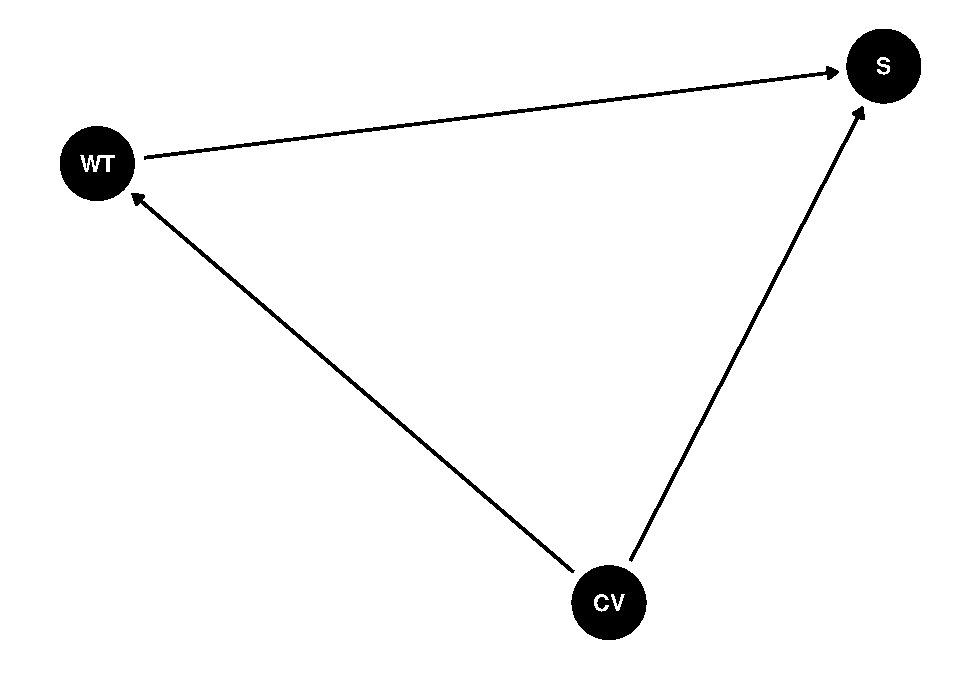
\includegraphics{final_prject_greß_files/figure-latex/unnamed-chunk-6-1.pdf}

Figure 2 shows the visual representation of the original third and
fourth hypotheses on the duration of civil conflicts. Again, the
identical control variables are included. In contrast to the hypotheses
on conflict severity, Moore expects a different effect direction of
weapon transfers, depending on whether the weapons are transferred to
rebels (conflict-shortening effect) or governments (conflict-prolonging
effect).

\begin{Shaded}
\begin{Highlighting}[]
\NormalTok{dag2 }\OtherTok{=} \FunctionTok{dagify}\NormalTok{(D }\SpecialCharTok{\textasciitilde{}}\NormalTok{ WT,}
\NormalTok{             D }\SpecialCharTok{\textasciitilde{}}\NormalTok{ CV,}
\NormalTok{             WT }\SpecialCharTok{\textasciitilde{}}\NormalTok{ CV)}
\FunctionTok{ggdag}\NormalTok{(dag) }\SpecialCharTok{+}  \FunctionTok{theme\_dag\_blank}\NormalTok{()}
\end{Highlighting}
\end{Shaded}

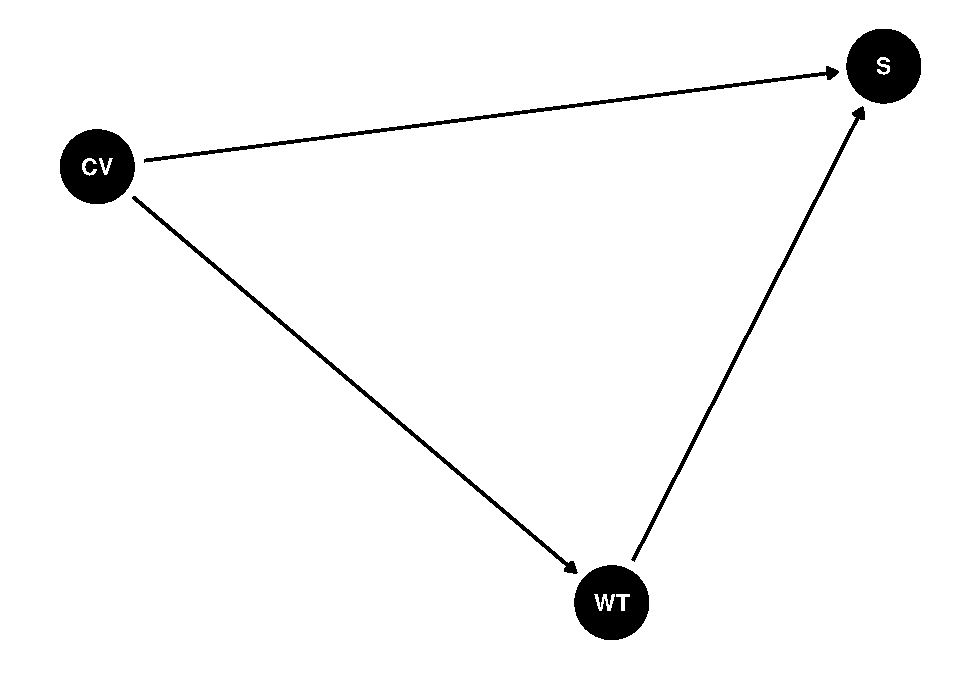
\includegraphics{final_prject_greß_files/figure-latex/unnamed-chunk-7-1.pdf}

\hypertarget{method-review}{%
\section{Method Review}\label{method-review}}

This section seeks to point out potential issues of the article by
Moore, both from a causal perspective as well as with regards to the
original coding decisions made by the author. An important constraint
for making causal statements in the whole domain of peace and conflict
studies is an endogeneity problem arising from both omitted variables
and simultaneity. Moore states that looking at weapon imports separately
from other types of third-party intervention solves potential
endogeneity issues. His main argument for this claim is that while other
forms of third-party intervention, such as sending physical troops,
might have a simultaneous relationship with increased casualties, the
effect direction between weapon imports and severity is unilateral. The
first part of this argument seems reasonable: Additional troops might
lead to an escalation of the conflict and a higher death toll, while a
higher death tool might simultaneously lead to the decision of sending
additional troops for supporting a certain conflict party. However, the
subsequent statement -- stating that weapon imports have the potential
to affect a conflict's severity but a reversed mechanism is not
conceivable - is questionable. Quite the contrary, it seems reasonable
to assume that especially the state party involved in a civil conflict
anticipates certain developments surrounding the threat of a conflict
outbreak. Similarly, governments might also -- in reaction to increasing
casualties -- strategically decide to import new weapons. This
expectation is supported by previous literature examining the
relationship between foreign aid and military expenditure
{[}collier2007unintended{]}. Hence, weapon imports could be both the
\emph{driver} and a \emph{result} of conflict severity and are not a
random governmental decision that can be seen independent of conflict
developments. This would imply an endogeneity issue due to simultaneous
causality (Bascle 2008). Following recent literature on endogeneity and
endogenous selection bias in social science applications, authors
pointed out that this endogeneity problem leads to biased and
inconsistent estimators Elwert and Winship (2014). Applied to the
analysis under examination, this subsequently implies that the
calculated coefficients of the respective weapon import variable are
biased and do not resemble the \emph{true} effect of weapon imports on a
conflict's severity. Although Moore concluded that this endogeneity
issue only arises when other forms of third-party interventions are
considered, more recent previous literature came to deviating
conclusions and pointed toward an endogenous relationship between weapon
imports and conflict trends (Mehrl and Thurner 2020, 1178). To
counteract this problem, Mehrl and Thurner introduce an instrumental
variable approach as a potential solution to this endogeneity problem.
The idea behind this approach is to include an additional variable (the
instrument) that is correlated with the respective independent variable
but not with the outcome and use it for providing exogenous variation in
the independent variable. Applied to this analysis, one would need to
include only one instrumental variable that is correlated with the
imports of MCW but not with conflict severity and duration.

Since Mehrl and Thurner examine both MCW and SALW, they include two
instrumental variables: for MCW imports, the authors include imports of
MCW not or only to a very limited extent suitable for intrastate
conflicts. This approach had been previously picked up by other
researchers (Pamp et al. 2018). Here, the authors argue that certain MCW
(air defence, submarines, ships, satellites) are rarely used in civil
conflicts and rather are used in interstate wars and are therefore a
suitable instrumental variable. Similarly, Mehrl and Thurner use
sporting and hunting weapons as an instrument for SALW imports, arguing
that these weapons are rarely used during conflict. They find that
governmental arms imports can render conflicts more violent, but only in
those cases where rebels are roughly equally strong.

As a preliminary result, it can be argued that Moore's methodological
framework has a clear weakness with regard to the endogeneity issue.
Looking at related, more recent literature, authors pointed toward this
problem and used instrumental variable approaches in order to account
for it. Using MCW that are not suitable for intrastate conflict as an
instrumental variable to account for endogeneity issues has been a
promising approach in recent literature and could be applied to Moore's
analysis to test the robustness of his results.

\hypertarget{coding-decisions-and-flaws}{%
\section{Coding decisions and flaws}\label{coding-decisions-and-flaws}}

Besides the more general endogeneity issue, another potential weakness
of the article is some of the operationalisations and measurements of
the key variables. One general difficulty of studies that examine the
severity of conflict is to implement a coherent and succinct measurement
of severity. Like many related studies, Moore uses the notion of
battle-related deaths as an indicator of a conflict's severity. Although
this is a common approach in related literature, there are some
individual adjustments that researchers can make that might
significantly influence the overall results. Regarding the overall
case-selection process, the potentially most impactful decision is to
determine at what threshold a conflict is considered in the analysis.
Moore follows a threshold of 900 battle-related deaths that happened
during the whole conflict. This is different from the general criteria
of UCDP for including a conflict, which is a threshold of 25
battle-related deaths per year of the conflict. Additionally, there also
is alternative literature and datasets which use a higher threshold
(more than 1,000 battle-related deaths per year, exemplarily in the
Correlates of War dataset). The general approach of UCDP is also
recommended by previous literature on methodological coding decisions
(Gates and Strand 2004): These authors argue that setting a lower
casualty threshold per year prevents systematic neglect of conflicts in
countries with generally lower population numbers and hence a selection
bias which is in favour of larger countries. However, the
yearly-measured death figure approach comes with a certain difficulty
addressed by Gates and Strand: Independently of the threshold set by the
researcher, some conflicts occasionally experience a drop in casualty
figures due to certain developments. When the number of battle-related
deaths drops under the specified threshold, the conflict is not
considered in the UCDP dataset anymore. From a theoretical perspective,
this could be especially problematic if the conflict is actually not
resolved (e.g.~due to a decisive defeat of one conflict party or a peace
agreement) but rather continues with a temporarily reduced intensity. If
the threshold is then exceeded again in a later year, UCDP would include
it as an inherently independent conflict, although it is likely that the
central actors and causes of war have stayed identical. In such cases,
it could be beneficial to recode the sample in a way that these
conflicts are treated as coherent. As proposed by Gates and Strand, one
possibility could be to code ``interrupted'' conflicts as coherent when
the period of inactivity is comparatively short. More concretely,
previous research suggested to code conflicts with interruptions that
lasted two years maximum as coherent and conflicts with longer inactive
periods as separate (Gates and Strand 2004).

As already introduced, Moore is not discussing such considerations in
his article since he is using an approach that accumulates the death
figures over time instead of considering every conflict year separately.
Although this partially circumvents the above-mentioned issues, this has
the disadvantage of a potentially systematic neglection of shorter
conflicts. Even if a conflict would experience high levels of violence
and battle-related deaths but stays below the threshold of 900
battle-related deaths and is then resolved quickly, the conflict would
not be considered in Moore's sample. Hence, these decisions are not only
affecting the general case number under examination but also the second
dependent variable of his article (duration). The article could already
be improved if the author would have provided a more transparent
discussion of the sample selection and/or the alternative approach of
concentrating on conflict years instead of overall death tolls for the
sample selection. Looking at related literature on weapon imports and
conflict trends, a sample selection based on UCDP's battle-related death
threshold per conflict year seems more widely used than Moore's
threshold, which seems quite arbitrary. Another disadvantage of this
varying case selection across studies is reduced comparability of
results since Moore's article might systematically leave out conflicts
that usually are included in analyses examining conflict intensity.

Ultimately, Mehrl and Thurner pointed toward a coding mistake in Moore's
article which potentially leads to flawed effect estimates. More
specifically, the weapon's import variable for governments was logged
twice. Obviously, the correct model specification intended to take the
log only once to account for the original distribution of the import
variable. However, Moore interprets the calculated estimates as if the
variable would have been logged only once, and finds significant effects
of governmental imports on conflict intensity. In order to verify the
claim of a flawed logarithmic transformation, let's briefly look at the
dataset used by Moore.

\begin{Shaded}
\begin{Highlighting}[]
\NormalTok{moore\_replication\_subset }\SpecialCharTok{\%\textgreater{}\%}
  \FunctionTok{select}\NormalTok{(starmimp5, lstarmimp5) }\SpecialCharTok{\%\textgreater{}\%} 
  \FunctionTok{head}\NormalTok{(., }\DecValTok{10}\NormalTok{)}
\end{Highlighting}
\end{Shaded}

\begin{verbatim}
##    starmimp5 lstarmimp5
## 1       7402  2.0938888
## 2        553         NA
## 3       1687  1.7308494
## 4        134  1.5887944
## 5          0  0.0000000
## 6         26  1.1285084
## 7       1872  1.7830609
## 10       242  0.5831981
## 11        29  1.1562691
## 12      1842  2.0101597
\end{verbatim}

As we can see, the values of the logged governmental arms import
variable that captures all imports that were made five years before the
outbreak of the conflict are flawed. The other import variables used by
Moore -- both for state imports during imports and both versions of the
rebel import variable -- are specified correctly. Hence, four of Moore's
models are affected: Models 3, 5, 7 and 9. In the next step of this
final project, I am correcting the coding error and replicating Moore's
models to be able to observe potential deviations.

\begin{tabular}{l|r|r|r|r}
\hline
term & estimate & std.error & statistic & p.value\\
\hline
(Intercept) & 9.3838393 & 3.1223547 & 3.0053726 & 0.0035792\\
\hline
new\_lstarmimp5 & 0.0770077 & 0.0933413 & 0.8250127 & 0.4119130\\
\hline
lrarmimp5 & 0.4076180 & 0.1391062 & 2.9302643 & 0.0044551\\
\hline
lnduration & 0.5616240 & 0.1369817 & 4.0999942 & 0.0001015\\
\hline
lnpop & -0.0758762 & 0.1513608 & -0.5012937 & 0.6175946\\
\hline
lnmilqual & 0.1851655 & 0.1301846 & 1.4223305 & 0.1589688\\
\hline
lngdp & -0.2428141 & 0.2046573 & -1.1864422 & 0.2390956\\
\hline
cw & 0.4658604 & 0.3155566 & 1.4763133 & 0.1439379\\
\hline
lnmountain & 0.0530812 & 0.1127414 & 0.4708226 & 0.6390985\\
\hline
democ & -0.9643369 & 0.4276543 & -2.2549447 & 0.0269778\\
\hline
ethnicpolar & -0.8644696 & 0.4191404 & -2.0624821 & 0.0425345\\
\hline
relpolar & 0.5002114 & 0.3594700 & 1.3915246 & 0.1680735\\
\hline
\end{tabular}

Looking at model 3 with the corrected specification of the governmental
imports variable and comparing it to the original estimates made by
Moore, we can see that both the coefficient value as well as the
significance has changed. While Moore concluded that governmental arms
imports before the conflict outbreak significantly increase the number
of battle-related deaths, the corrected version implies that there is no
identifiable effect. Thus, the significant effect of governmental arms
imports was due to the coding mistake and does not imply a real effect.
Besides the changed effect of the governmental imports variable, the
other coefficients of the included variables also changed. However, the
effect size of rebel weapon imports, which was specified correctly by
Moore, only changed to a minor extent and stayed in the same direction.
Also, the significance of these variables was not affected by replacing
the flawed governmental import variable.

\begin{Shaded}
\begin{Highlighting}[]
\NormalTok{model5 }\OtherTok{\textless{}{-}} \FunctionTok{lm}\NormalTok{(lnbdb }\SpecialCharTok{\textasciitilde{}}\NormalTok{ new\_lstarmimp5 }\SpecialCharTok{+}\NormalTok{ lrarmimp5 }\SpecialCharTok{+}\NormalTok{ lnduration }\SpecialCharTok{+}\NormalTok{ lnpop }\SpecialCharTok{+}\NormalTok{ lnmilqual }\SpecialCharTok{+}\NormalTok{ lngdp }\SpecialCharTok{+}\NormalTok{ cw }\SpecialCharTok{+}\NormalTok{ lnmountain }\SpecialCharTok{+}\NormalTok{ democ }\SpecialCharTok{+}\NormalTok{ ethnicpolar }\SpecialCharTok{+}\NormalTok{ relpolar }\SpecialCharTok{+}\NormalTok{ intervention, }\AttributeTok{data =}\NormalTok{ moore\_replication\_subset)}

\FunctionTok{summary}\NormalTok{(model5)}
\end{Highlighting}
\end{Shaded}

\begin{verbatim}
## 
## Call:
## lm(formula = lnbdb ~ new_lstarmimp5 + lrarmimp5 + lnduration + 
##     lnpop + lnmilqual + lngdp + cw + lnmountain + democ + ethnicpolar + 
##     relpolar + intervention, data = moore_replication_subset)
## 
## Residuals:
##     Min      1Q  Median      3Q     Max 
## -2.1456 -0.8605  0.0289  0.6418  2.6936 
## 
## Coefficients:
##                Estimate Std. Error t value Pr(>|t|)    
## (Intercept)     6.33458    3.07428   2.061 0.042772 *  
## new_lstarmimp5  0.07619    0.08775   0.868 0.387967    
## lrarmimp5       0.42639    0.13089   3.258 0.001681 ** 
## lnduration      0.46606    0.13192   3.533 0.000703 ***
## lnpop           0.06102    0.14809   0.412 0.681487    
## lnmilqual       0.14747    0.12290   1.200 0.233927    
## lngdp          -0.15560    0.19416  -0.801 0.425415    
## cw              0.32318    0.29971   1.078 0.284310    
## lnmountain      0.08385    0.10639   0.788 0.433026    
## democ          -0.98482    0.40208  -2.449 0.016614 *  
## ethnicpolar    -0.78179    0.39480  -1.980 0.051300 .  
## relpolar        0.48524    0.33796   1.436 0.155163    
## intervention    0.94480    0.28321   3.336 0.001317 ** 
## ---
## Signif. codes:  0 '***' 0.001 '**' 0.01 '*' 0.05 '.' 0.1 ' ' 1
## 
## Residual standard error: 1.109 on 76 degrees of freedom
##   (12 Beobachtungen als fehlend gelöscht)
## Multiple R-squared:   0.58,  Adjusted R-squared:  0.5137 
## F-statistic: 8.745 on 12 and 76 DF,  p-value: 3.357e-10
\end{verbatim}

In model 5, Moore additionally included third-party interventions to
evaluate potential effects on the import variable. Again, he found an
even stronger effect pointing towards increased conflict severity caused
by governmental weapon imports. The corrected version of the model shows
again that this finding was due to the coding mistake and does not hold
when the variable is correctly specified. As in model 3, the coefficient
of governmental arms imports turns insignificant. Hence, the correct
interpretation of the model would conclude that there is no systematic,
identifiable pattern of how governmental arms imports are correlated
with the development of conflict intensity. Again, the originally
identified, significant effect of rebel arms import is not affected by
the inclusion of the corrected variable.

Having looked at the two corrected models that examined the influence of
weapon imports on conflict severity, we can now revise Moore's original
hypotheses in that regard. In hypothesis 2, Moore stated that MCW
transfers to governments or states would increase the severity of civil
conflicts. The incorrect specification of the import variable confirmed
this hypothesis when long-term imports were considered. The replication
of the analysis with the corrected version showed that these effects are
no longer significant. Combined with the other models of Moore's
analysis, it becomes clear that governmental arms imports did not have a
significant impact on conflict duration in any of the specified models.
Thus, Moore's original second hypothesis must be declined since there is
no systematic relationship between weapon imports made by governments
and the severity of civil conflicts. On the other hand, Moore's results
regarding the effect of weapon transfers to rebels, which are included
in hypothesis 1, still hold.

After discussing the corrected results regarding conflict severity, also
the models and hypotheses on conflict duration need to be reexamined.
Again, two models were affected by the incorrect variable specification:
model 7, which examines long-term imports on civil war duration, and
model 9, which does the same but also includes the third-party
intervention variable.

\begin{Shaded}
\begin{Highlighting}[]
\NormalTok{moore\_replication\_subset}\SpecialCharTok{$}\NormalTok{status }\OtherTok{=} \DecValTok{1}

\NormalTok{model7 }\OtherTok{\textless{}{-}} \FunctionTok{coxph}\NormalTok{( }\FunctionTok{Surv}\NormalTok{(duration, status) }\SpecialCharTok{\textasciitilde{}}\NormalTok{ new\_lstarmimp5 }\SpecialCharTok{+}\NormalTok{ lrarmimp5 }\SpecialCharTok{+}\NormalTok{ lnpop }\SpecialCharTok{+}\NormalTok{ lnmilqual }\SpecialCharTok{+}\NormalTok{ lngdp }\SpecialCharTok{+}\NormalTok{ cw }\SpecialCharTok{+}\NormalTok{ lnmountain }\SpecialCharTok{+}\NormalTok{ democ  }\SpecialCharTok{+}\NormalTok{ ethnicpolar }\SpecialCharTok{+}\NormalTok{ relpolar, }\AttributeTok{data =}\NormalTok{ moore\_replication\_subset)}

\FunctionTok{summary}\NormalTok{(model7)}
\end{Highlighting}
\end{Shaded}

\begin{verbatim}
## Call:
## coxph(formula = Surv(duration, status) ~ new_lstarmimp5 + lrarmimp5 + 
##     lnpop + lnmilqual + lngdp + cw + lnmountain + democ + ethnicpolar + 
##     relpolar, data = moore_replication_subset)
## 
##   n= 89, number of events= 89 
##    (12 Beobachtungen als fehlend gelöscht)
## 
##                     coef exp(coef)  se(coef)      z Pr(>|z|)    
## new_lstarmimp5 -0.359707  0.697881  0.087394 -4.116 3.86e-05 ***
## lrarmimp5      -0.023777  0.976503  0.119382 -0.199  0.84213    
## lnpop           0.410886  1.508153  0.142906  2.875  0.00404 ** 
## lnmilqual       0.008855  1.008894  0.126296  0.070  0.94410    
## lngdp           0.296986  1.345796  0.191739  1.549  0.12140    
## cw             -0.126806  0.880904  0.318706 -0.398  0.69072    
## lnmountain     -0.099017  0.905727  0.093041 -1.064  0.28723    
## democ          -0.466238  0.627358  0.415912 -1.121  0.26229    
## ethnicpolar     0.669817  1.953879  0.392947  1.705  0.08827 .  
## relpolar       -0.039429  0.961338  0.345335 -0.114  0.90910    
## ---
## Signif. codes:  0 '***' 0.001 '**' 0.01 '*' 0.05 '.' 0.1 ' ' 1
## 
##                exp(coef) exp(-coef) lower .95 upper .95
## new_lstarmimp5    0.6979     1.4329    0.5880    0.8283
## lrarmimp5         0.9765     1.0241    0.7728    1.2339
## lnpop             1.5082     0.6631    1.1397    1.9957
## lnmilqual         1.0089     0.9912    0.7877    1.2923
## lngdp             1.3458     0.7431    0.9242    1.9597
## cw                0.8809     1.1352    0.4717    1.6452
## lnmountain        0.9057     1.1041    0.7547    1.0869
## democ             0.6274     1.5940    0.2776    1.4176
## ethnicpolar       1.9539     0.5118    0.9045    4.2206
## relpolar          0.9613     1.0402    0.4886    1.8916
## 
## Concordance= 0.69  (se = 0.03 )
## Likelihood ratio test= 32.77  on 10 df,   p=3e-04
## Wald test            = 31.81  on 10 df,   p=4e-04
## Score (logrank) test = 34.05  on 10 df,   p=2e-04
\end{verbatim}

As we can see from the Cox regression output, the coefficients for state
arms imports change again. However, the direction of the effect stays
the same and also the statistical significance is not affected. When the
flawed estimates from Moore's article and the corrected ones above are
compared, we can see that the corrected estimate are somewhat smaller
than Moore's original estimate for governmental weapon imports on civil
conflict duration (-1.44). Subsequently, Moore's hypothesis that MCW
transfers to governments are related to longer enduring conflicts is
still supported, but the effect seems to be marginally weaker.

\begin{Shaded}
\begin{Highlighting}[]
\NormalTok{model9 }\OtherTok{\textless{}{-}} \FunctionTok{coxph}\NormalTok{(}\FunctionTok{Surv}\NormalTok{(duration, status) }\SpecialCharTok{\textasciitilde{}}\NormalTok{ new\_lstarmimp5 }\SpecialCharTok{+}\NormalTok{ lrarmimp5 }\SpecialCharTok{+}\NormalTok{ lnpop }\SpecialCharTok{+}\NormalTok{ lnmilqual }\SpecialCharTok{+}\NormalTok{ lngdp }\SpecialCharTok{+}\NormalTok{ cw }\SpecialCharTok{+}\NormalTok{ lnmountain }\SpecialCharTok{+}\NormalTok{ democ }\SpecialCharTok{+}\NormalTok{ ethnicpolar }\SpecialCharTok{+}\NormalTok{ relpolar }\SpecialCharTok{+}\NormalTok{ intervention, }\AttributeTok{data =}\NormalTok{ moore\_replication\_subset)}

\FunctionTok{summary}\NormalTok{(model9)}
\end{Highlighting}
\end{Shaded}

\begin{verbatim}
## Call:
## coxph(formula = Surv(duration, status) ~ new_lstarmimp5 + lrarmimp5 + 
##     lnpop + lnmilqual + lngdp + cw + lnmountain + democ + ethnicpolar + 
##     relpolar + intervention, data = moore_replication_subset)
## 
##   n= 89, number of events= 89 
##    (12 Beobachtungen als fehlend gelöscht)
## 
##                    coef exp(coef) se(coef)      z Pr(>|z|)    
## new_lstarmimp5 -0.34437   0.70867  0.08456 -4.072 4.65e-05 ***
## lrarmimp5      -0.06532   0.93677  0.12023 -0.543   0.5869    
## lnpop           0.31675   1.37265  0.14968  2.116   0.0343 *  
## lnmilqual       0.06373   1.06581  0.13184  0.483   0.6288    
## lngdp           0.22450   1.25169  0.18873  1.190   0.2342    
## cw              0.04048   1.04131  0.32717  0.124   0.9015    
## lnmountain     -0.11740   0.88923  0.09395 -1.250   0.2115    
## democ          -0.53693   0.58454  0.43314 -1.240   0.2151    
## ethnicpolar     0.62991   1.87743  0.40234  1.566   0.1174    
## relpolar       -0.04894   0.95224  0.35053 -0.140   0.8890    
## intervention   -0.57905   0.56043  0.27171 -2.131   0.0331 *  
## ---
## Signif. codes:  0 '***' 0.001 '**' 0.01 '*' 0.05 '.' 0.1 ' ' 1
## 
##                exp(coef) exp(-coef) lower .95 upper .95
## new_lstarmimp5    0.7087     1.4111    0.6004    0.8364
## lrarmimp5         0.9368     1.0675    0.7401    1.1857
## lnpop             1.3727     0.7285    1.0237    1.8406
## lnmilqual         1.0658     0.9383    0.8231    1.3801
## lngdp             1.2517     0.7989    0.8647    1.8120
## cw                1.0413     0.9603    0.5484    1.9773
## lnmountain        0.8892     1.1246    0.7397    1.0690
## democ             0.5845     1.7108    0.2501    1.3662
## ethnicpolar       1.8774     0.5326    0.8533    4.1308
## relpolar          0.9522     1.0502    0.4790    1.8929
## intervention      0.5604     1.7843    0.3290    0.9546
## 
## Concordance= 0.704  (se = 0.03 )
## Likelihood ratio test= 37.25  on 11 df,   p=1e-04
## Wald test            = 35.45  on 11 df,   p=2e-04
## Score (logrank) test = 38.22  on 11 df,   p=7e-05
\end{verbatim}

Ultimately, the corrected version of model 9 is also quite similar to
Moore's original finding: The governmental arms import variable is still
significant and in the expected direction, but the effect is again not
as strong as originally found.

\hypertarget{conclusion-and-outlook}{%
\section{Conclusion and Outlook}\label{conclusion-and-outlook}}

This final project examined Moore's article on the relationship between
weapons imports to rebels and governments and conflict severity and
duration. Besides briefly summarizing Moore's key results, the main goal
of this project was to provide a methodological critique and to provide
a corrected replication of his models. I identified three key
methodological weaknesses of the original article: First, Moore states
that there is no endogeneity problem with regard to the relationship
between weapon imports and conflict severity. He argues that such a
problem only arises when other forms of third-party interventions are
considered, but that the causal relationship between imports and
severity is one-sided. However, it seems conceivable that states import
weapons both in anticipation and as a reaction to conflict developments.
Subsequently, a simultaneous relationship and the following endogeneity
issue would be present. This has already been addressed by more recent
literature {[}mehrl2020military{]}, which uses an instrumental variable
approach as a countermeasure. In a future application, Moore's analysis
could be replicated with an additional instrumental variable for the
import of MCW. If the same instrument as in Mehrl/Thurner is included
(MCW non-suitable for intrastate conflict), the same data source (SIPRI)
that is already providing the data on weapon imports can be used. SIPRI
allows for distinguishing between certain types of MCW, and future
research could therefore separate between suitable and non-suitable MCW.
However, a potential challenge could be the hypotheses that examine
rebels' imports, since rebels rarely import non-suitable MCW in general.
The second problem was the measurement of the main dependent variables,
conflict severity and duration as well as the sample selection. As
discussed, Moore used a seemingly arbitrary casualty threshold of 900
battle-related deaths during the entire conflict as a selection
criterium. However, the common approach is to make the existence of a
conflict depend on the battle-related deaths per year (the common
threshold is 25 for smaller conflicts and 1,000 for civil wars). Moore's
approach potentially leads to a systematic exclusion of short conflicts
with a high peak in casualties at the beginning and a fast termination
afterwards. Moreover, the deviation from the widely used case selection
criteria reduces the comparability of Moore's results. Lastly, previous
literature already pointed toward a coding mistake regarding the
long-term governmental arms imports variable in Moore's analysis (Mehrl
and Thurner 2020). Instead of log-transforming the variable only once,
the authors accidentally log-transformed it twice. Obviously, this
mistake biased the coefficients for the respective variable. In this
analysis, I replicated the affected models from Moore's analysis with a
corrected version of the import variable. As a result, the originally
significant results regarding the effect of governmental weapon imports
on conflict severity turned insignificant. Subsequently, the analysis
did not find a systematic relationship between governmental arms imports
and the development of battle-related deaths. On the other hand, the
results regarding conflict duration seem to be only affected to a minor
extent: the relationship stays significant and in the same direction as
in the original analysis, finding that governmental arms imports are
correlated with longer civil conflicts. The only difference is a slight
reduction in the strength of the effect.

\hypertarget{refs}{}
\begin{CSLReferences}{1}{0}
\leavevmode\vadjust pre{\hypertarget{ref-bascle2008controlling}{}}%
Bascle, Guilhem. 2008. {``Controlling for Endogeneity with Instrumental
Variables in Strategic Management Research.''} \emph{Strategic
Organization} 6 (3): 285--327.

\leavevmode\vadjust pre{\hypertarget{ref-elwert2014endogenous}{}}%
Elwert, Felix, and Christopher Winship. 2014. {``Endogenous Selection
Bias: The Problem of Conditioning on a Collider Variable.''}
\emph{Annual Review of Sociology} 40: 31--53.

\leavevmode\vadjust pre{\hypertarget{ref-gates2004modeling}{}}%
Gates, Scott, and Håvard Strand. 2004. {``Modeling the Duration of Civil
Wars: Measurement and Estimation Issues.''} In \emph{Presentation at the
Joint Session of Workshops of the ECPR, Uppsala}.

\leavevmode\vadjust pre{\hypertarget{ref-glymour2016causal}{}}%
Glymour, Madelyn, Judea Pearl, and Nicholas P Jewell. 2016. \emph{Causal
Inference in Statistics: A Primer}. John Wiley \& Sons.

\leavevmode\vadjust pre{\hypertarget{ref-lacina2006explaining}{}}%
Lacina, Bethany. 2006. {``Explaining the Severity of Civil Wars.''}
\emph{Journal of Conflict Resolution} 50 (2): 276--89.

\leavevmode\vadjust pre{\hypertarget{ref-mehrl2020military}{}}%
Mehrl, Marius, and Paul W Thurner. 2020. {``Military Technology and
Human Loss in Intrastate Conflict: The Conditional Impact of Arms
Imports.''} \emph{Journal of Conflict Resolution} 64 (6): 1172--96.

\leavevmode\vadjust pre{\hypertarget{ref-moore2012selling}{}}%
Moore, Matthew. 2012. {``Selling to Both Sides: The Effects of Major
Conventional Weapons Transfers on Civil War Severity and Duration.''}
\emph{International Interactions} 38 (3): 325--47.

\leavevmode\vadjust pre{\hypertarget{ref-pamp2018build}{}}%
Pamp, Oliver, Lukas Rudolph, Paul W Thurner, Andreas Mehltretter, and
Simon Primus. 2018. {``The Build-up of Coercive Capacities: Arms Imports
and the Outbreak of Violent Intrastate Conflicts.''} \emph{Journal of
Peace Research} 55 (4): 430--44.

\end{CSLReferences}

\end{document}
